\section{Performance Impact of Constant Expressions}\label{sec:perf}

One of the essential features of \Noarr{} is that the first-class structures propagate along with their templated types, allowing us to embed statically defined properties (most importantly, the constant dimensions of the structure) into the type itself. Therefore, the compiler can employ optimizations like compile-time evaluation of constant expressions or exact-sized loop unrolling, which might lead to more efficient execution or even automated vectorization. These optimizations rarely produce a game-changing improvement in performance; thus, the programmers often overlook them. However, utilization of \Noarr{} structure will introduce them naturally so the result code could run faster without any additional effort whilst maintaining other benefits like memory allocation decoupling or coding in a layout-agnostic manner.

To present the main idea, let us have an array $A$ of $N$ vectors in $\mathbb{R}^D$ where $N$ is a variable, and $D$ is a constant\footnote{If the code needs to handle several different dimensionalities $D$, it will be compiled for each $D$ independently thanks to the power of C++ templates.}. We want to compute the Euclidean distance between every vector in the array and given vector $q$ (e.g., to find $k$ nearest vectors, which is quite a typical task in many data-processing problems):

\begin{minted}[fontsize=\scriptsize]{c++}
  for (size_t i = 0; i < N; ++i) {
    float dist = 0.0f;
    for (size_t d = 0; d < D; ++d) {
      float diff = A[i*D + d] - q[d];
      dist += diff * diff;
    }
    dist = std::sqrtf(dist); // ...
  }
\end{minted}

When $D$ is a constant, the compiler could unroll the loop entirely without additional branches. It might even attempt to unroll the outer loop if $D$ is sufficiently small. The speedup achieved by having constant $D$ may easily reach factor $3\times$ for very small values of $D$ (e.g., $D=2$)\footnote{If we measure only the Euclidean distance computation.}.


% -----------------------------------------------------------------------------
\subsection{Indexing performance}
% -----------------------------------------------------------------------------

To demonstrate the impact of \Noarr{} structures, we have selected a 3D stencil problem as an example. Stencil is a simple function computed iteratively for every element of a regular grid. We have used an averaging stencil executed on a 3D grid which could be used as an approximative simulation of gas diffusion, for instance. Our objective is to emphasize the difference between situations when the grid dimensions are constant (at compile time) and when they are determined at runtime.

The main code of the stencil is in Listing~\ref{lst:stencil_base}. Run-time variables \texttt{size\_x}, \texttt{size\_y}, and \texttt{size\_z} denote the dimensions of the cube. The first part of this experiment aims at exposing only the compile-time optimizations of index computations, so we ensure that no optimizations related to constant dimensions are performed. Please note that the loops do not visit points residing on the faces of the grid so that we can ignore the border cases of the stencil function; thus, there are no branches in the code which leads to simpler and more stable measurement. 

\begin{listing}[h]
    \vspace{-10pt}
    \inputmintedcpp{noarr/code-snippets/stencil_base.cpp}
    \vspace{-20pt}
    \caption{Main stencil for-loop}
    \label{lst:stencil_base}
\end{listing}

A na\"{i}ve C-like implementation of the internal \texttt{stencil} function is presented in Listing \ref{lst:stencil_trivial}. It uses the same variables in the loop to index the data pointers, preventing the compiler from doing more elaborate compile-time optimizations. This code is used as a baseline for the performance comparison.

\begin{listing}[h]
    \vspace{-10pt}
    \inputmintedcpp{noarr/code-snippets/stencil_trivial.cpp}
    \vspace{-20pt}
    \caption{Na\"{i}ve implementation of stencil function}
    \label{lst:stencil_trivial}
\end{listing}
\vspace{-10pt}

Making the dimensions constant may help the compiler to generate more optimal code. In C++, this can be achieved simply by defining the \texttt{size\_*} variables as \texttt{constexpr}; however, such constants need to be declared at the global level, which significantly undermines any encapsulation or reusability of the code. Better way is to use fix-sized containers like \texttt{std::array} and make the stencil code templated so it can be used with any compatible containers (including \texttt{std::vector}).

\begin{listing}[h]
  \vspace{-10pt}
  \inputmintedcpp{noarr/code-snippets/stencil_noarr.cpp}
  \vspace{-20pt}
  \caption{\Noarr{} implementation of stencil with constant-sized \texttt{array}}
  \label{lst:stencil_noarr}
\end{listing}
\vspace{-10pt}

\Noarr{} provides a fixed layout structure \texttt{array}, which fulfills a similar role, but it can be easily integrated into more complex nested structures (even with custom layouts). Listing \ref{lst:stencil_noarr} presents the internal \texttt{stencil} rewritten for \Noarr{}. The dimensions of the grid are no longer passed as variables, but they are embedded in the type of the \texttt{bag} structure as constants. Line $1$ shows the assembling of the layout structure using a predefined \texttt{array} template.

To evaluate the performance, we have selected a grid of a specific size ($2^{20} \times 32 \times 32$) which confines the meaning of the diffuse simulation for a specific environment (e.g., gas in a pipe). The main reason is that the performance improvement caused by the compile-time optimizations is difficult to measure on regular structures since it takes only a small portion of overall time (especially when the computation causes many cache misses). This shape requires more index computations relative to other operations, making the difference more pronounced in the measurements.

\begin{figure}[h]
  \vspace{-10pt}
	\centering
	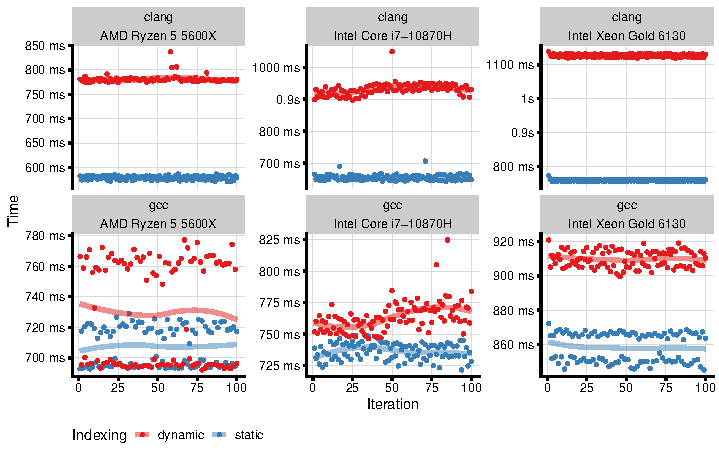
\includegraphics{noarr/plots/stencil.pdf}
	\caption{Wall times of $100$ stencil iterations (plotted lines represent the local regression of the measured times)}
	\label{fig:stencil}
  \vspace{-10pt}
\end{figure}

Figure \ref{fig:stencil} shows the comparison results of the two presented stencil implementations on three platforms using two compilers. The benefits of compile-time optimizations are visible on every platform and with both tested compilers, albeit there is only a small difference in some configurations. The details regarding the experimental methodology are summarized in Appendix~\ref{appendix:methodology}.


% -----------------------------------------------------------------------------
\subsection{Constant-loops optimizations}
% -----------------------------------------------------------------------------

The second part of this experiment extends the compile-time optimizations to the nested stencil grid loops. It requires replacing \texttt{size\_*} variables in the main loops (Listing \ref{lst:stencil_base}) with constants (i.e., \texttt{constexpr} or template arguments) so the compiler has enough information to perform exact loop-unrolling and better vectorization-related optimizations.

\begin{listing}[h]
  \vspace{-10pt}
  \inputmintedcpp{noarr/code-snippets/stencil_base_bag.cpp}
  \vspace{-20pt}
  \caption{Updated stencil for-loop with \texttt{bag} structure}
  \label{lst:stencil_base_bag}
\end{listing}
\vspace{-10pt}

However, converting these variables to constants may be quite tedious, especially if we want the code to be generic for both constant and non-constant scenarios. This particular issue can be easily overcome by utilization of \Noarr{} \texttt{bag} structures. Having the layout information encoded both in the structure type and the object, method \texttt{get\_length} can query dimension sizes and returns a constant or variable based on the layout specification, all this being decided at compile time. The grid loop function from Listing \ref{lst:stencil_base} needs to be rewritten as demonstrated in Listing~\ref{lst:stencil_base_bag}.

\begin{figure}[H]
  \vspace{-10pt}
	\centering
	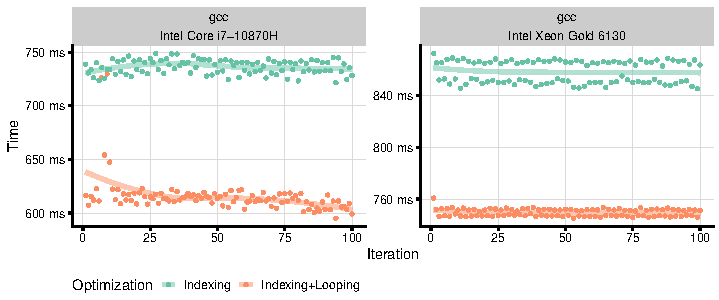
\includegraphics{noarr/plots/stencil_loop.pdf}
	\caption{Stencil execution times of two optimizations --- compile-time \emph{indexing} and the addition of constant-induced loop unrolling (\emph{indexing+looping})}
	\label{fig:stencil_wloop}
  \vspace{-10pt}
\end{figure}

Figure \ref{fig:stencil_wloop} presents the performance improvements of exposing constant variables to the grid iteration loop. We have included only measurements of programs compiled by \texttt{gcc} since \texttt{clang} was not able to take advantage of the constant values when they are passed through the \texttt{bag} structure interface.
